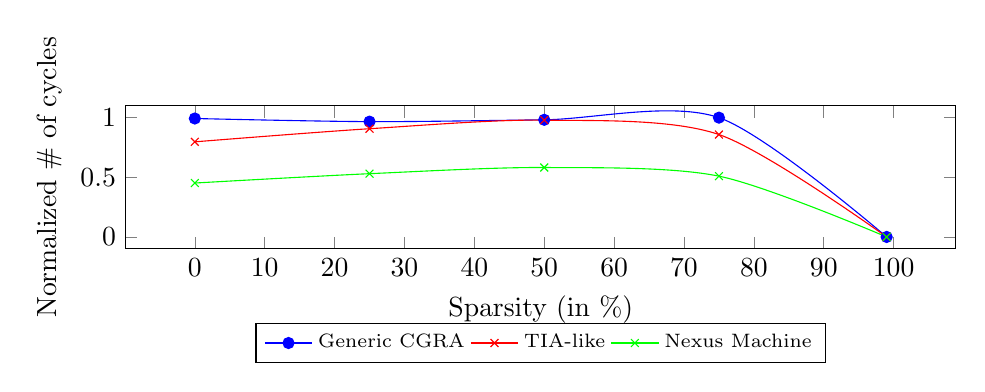
\begin{tikzpicture}
\begin{axis}[
    width=\columnwidth, height=3.4cm,
    xlabel=Sparsity (in \%),
    ylabel=Normalized \# of cycles,
    %xlabels at=edge bottom,
    %xticklabels at=edge bottom,
    %typeset ticklabels with strut,
    legend columns=4,
    legend columns=4,
    legend style={at={(0.5,-0.8,1.15)},
    anchor=south, font=\scriptsize},
    %xticklabels from table={graphs/data/spmv_performance.data}{Sparsity},
    ]
    
\addplot[smooth,mark=*,blue] plot coordinates {
    (99,0)
    (75,1)
    (50,0.981899265)
    (25,0.966552991)
    (0,0.992785939)
};
\addlegendentry{Generic CGRA}

\addplot[smooth,color=red,mark=x]
    plot coordinates {
    (99,0)
    (75,0.858473242)
    (50,0.978926198)
    (25,0.907179084)
    (0,0.797306751)
};
\addlegendentry{TIA-like}

\addplot[smooth,color=green,mark=x]
    plot coordinates {
    (99,0)
    (75,0.509706191)
    (50,0.582021686)
    (25,0.530342777)
    (0,0.451949983)
};
\addlegendentry{Nexus Machine}

\end{axis}
\end{tikzpicture}